\subsection*{Explicación}
Al analizar el comportamiento del JKlatch observamos que este invierte los valores de q y nq cuando c=1, j=1 y k=1. Asigna los valores de j a q y de k a nq cuando j y k son diferentes ,y c=1. Y mantiene los valores previos de q y nq cuando j=0 y k=0 ,y c=1. Al igual que el T-latch en la implementacion le agregue un delay para evitar oscilaciones infinitas.

\subsection*{Tabla de verdad}
\begin{figure}[h]
    \centering
    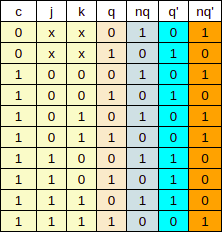
\includegraphics{fotos/TruthTable/arki-lab2-TT_jklatch.png}
\end{figure}
\subsection*{Mapa de Karnaugh}
\begin{figure}[h]
    \centering
    \includegraphics{fotos/kmaps/arki-lab2-kmap_jklatch.png}
\end{figure}
%\subsection*{Ecuaciones booleanas}

\newpage
\subsection*{Resultados}
\begin{figure}[h]
    \centering
    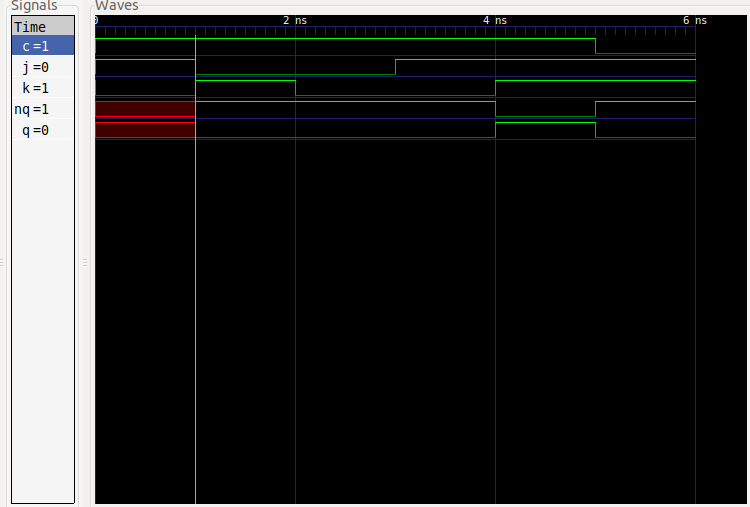
\includegraphics[scale=0.5]{fotos/resultados/arki-lab2-R_jklatch.png}
\end{figure}